% Este arquivo .tex será incluído no arquivo .tex principal. Não é preciso
% declarar nenhum cabeçalho

\section{Bem-vindo à academia}

Não, bixo, você não vai comer frango com batata doce no bandeco e ir puxar ferro
na FEF todo dia.  

Academia é o nome que se dá à comunidade internacional de pesquisadores e
estudantes de ensino superior, atuando em todas as áreas do
conhecimento. Geralmente centrada ao redor de universidades, porém organizações
públicas e privadas e também empresas fazem parte.

A Unicamp está muito bem situada no cenário acadêmico, sendo a responsável por
15\% da produção científica brasileira, e tendo inúmeros pesquisadores de renome
internacional, então não vão faltar oportunidades para você entrar nesse mundo.

\subsection{Iniciação Científica}

A Iniciação Científica é um tempo para o aluno de graduação (você, no caso) ter
uma experiência acadêmica mais séria, sentir um pouco como é o clima de
pesquisa. Interessou? O que fazer? Calma, você mal entrou na Universidade.
Geralmente, o que se faz é conversar com o professor da área com a qual você se
identifica mais (criptografia, teoria da computação, processamento de imagens,
inteligência artificial etc.) e ver se ele está desenvolvendo algum projeto
interessante naquela área, ou propor para ele alguma ideia sua mesmo.  Depois
você começa a estudar para redigir um projeto e encaminhá-lo para alguma
instituição de fomento à pesquisa (CNPq ou FAPESP), pedindo uma bolsa de
Iniciação Científica. A FAPESP paga em torno de R\$520,00 e aceita pedidos de
bolsa em qualquer período do ano. O CNPq paga aproximadamente R\$400,00, e o
período para inscrição de projetos é geralmente em junho e novembro. No primeiro
semestre geralmente é bem mais difícil achar algum professor da área que você se
interessa, aliás, é bem difícil saber a área com a qual você se identifica, pois
você mal começou o curso e não conhece muito do que se estuda em Computação,
muito menos os professores. Mas tenha paciência, agora parece tudo muito
complicado, mas com o tempo as coisas vão ficando mais simples. Se você
realmente tiver uma sede insaciável de conhecer o meio da pesquisa, procure o
seu professor de MC102, ele pode te orientar a respeito.

\begin{figure}[h!]
    \centering
    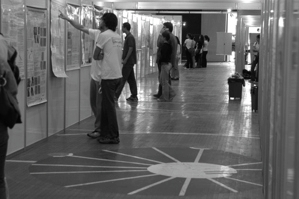
\includegraphics[width=.45\textwidth]{img/unicamp/congresso.jpg}
    \caption*{Congresso de Iniciação Científica da Unicamp}
\end{figure}

Outra coisa interessante a respeito da Iniciação Científica é que, se você
conseguir bolsa (o que não é muito difícil), pode pegar a disciplina MC040 e
posteriormente MC041 (2 semestres), cada uma com 12 créditos, e geralmente se
tira notas altas nessas disciplinas. Ou seja, são 24 créditos praticamente ``de
bandeja'' para aumentar o seu CR, ou ajudar a recuperá-lo, caso esteja no fundo
do poço. Note bem as aspas. Os trabalhos de Iniciação Científica geralmente
consomem muito tempo de estudo e dedicação, não vá pensando que é moleza não.

Na FEEC você pode conseguir as matérias de Iniciação (EA002 até EA005) mesmo sem
bolsa, mas você ainda assim vai precisar de um orientador. Lá a Iniciação
Científica também substitui o estágio, mas não tem equivalência com as do IC.

\subsection{Intercâmbio}

A Unicamp é uma das universidades brasileiras que têm maior prestígio fora do
país e a VRERI-Unicamp (Vice-Reitoria Executiva de Relações Internacionais,
antigo CORI), IC e FEEC têm vários acordos bilaterais de intercâmbio. Então,
para você que quer dar um salto em algum idioma, conheceroutras culturas e
sentir na pele a aventura de ser estrangeiro, comece a se preparar desde já.

Muita gente costumava pegar intercâmbio pelo Ciência Sem Fronteiras, mas ele foi
congelado pelo Governo Federal em 2015. É possível que ele volte no futuro, mas
não muito provável, dada a situação financeira atual do Governo. Ainda existem
boas opções pra quem gostaria de pegar um intercâmbio, mas ficou muito mais
difícil.

A França hoje recebe um número razoável de estudantes de computação, devido a
acordos que a Unicamp tem com os INSA e com as Écoles Centrales e também graças
a bolsas de estudo oferecidas pela Capes e pelo governo francês. Os intercâmbios
para a França são bem mais concorridos que o Ciência sem Fronteiras, pois são na
modalidade de duplo diploma (você se forma pela Unicamp e pela instituição
francesa), há um processo seletivo envolvendo uma entrevista, e vai durar mais
tempo, dois anos ou mais, numa instituição de prestígio como a École
Polytechnique, por exemplo.

No site da VRERI existem oportunidades para ir para Estados Unidos, Japão,
América Latina, Alemanha, Espanha etc., muitos com boas bolsas de estudo ou com
incentivos que valem a pena caso você tenha um pouco de grana para se sustentar
no início. Visite sempre o site da VRERI e participe das reuniões que ela faz,
pois ficar ligado é a chave para conseguir encontrar uma boa
oportunidade. Existem outras opções de intercâmbio, como a AIESEC, que promove
um intercâmbio para estágios no exterior. Se seu interesse é mais profissional,
procure se informar.

\begin{quote}
``Mas vale a pena? Poxa, vou atrasar meu curso, ficarei deslocado de turma, vou
ficar em um país estranho, para quê? Acho que não vale a pena{\dots}''
\end{quote}
Vamos começar pelos motivos profissionais: ter no currículo que você fala uma
língua estrangeira fluentemente devido à sua imersão no país é algo muito
valorizado pelas empresas, além do fato que o pessoal do RH vai ver que você tem
capacidade de se virar sozinho, uma vez que não é tão óbvio sair do país e
recomeçar sua vida fora. Você não atrasará tanto seu curso, pois a Unicamp conta
com um sistema de equivalências de matérias, e se você escolher bem pode fazer
matérias que serão convalidadas na Unicamp. Agora, o que realmente é importante:
você está na faculdade, está na hora de deixar o colo da mamãe e partir para o
mundo! A experiência de conhecer outras culturas, criar laços de amizade
internacionais, viajar por terras desconhecidas não tem preço! Pense que é no
seu tempo de facul que terá oportunidade de fazer uma aventura destas, não
desperdice.

Se você abriu um sorriso e pensa que está preparado para sair do país, comece a
estudar, bixo! Não que ter uma boa nota seja a única forma de conseguir uma vaga
em uma bolsa de estudos, mas com certeza é a mais fácil.  Busque atirar em todas
as frentes, mantenha seu CR num bom nível, busque conhecer organismos como
AIESEC e procure grupos de trabalho (no IC existem vários) que podem levar
alunos ao exterior. Boa sorte!

Se você realmente se interessou, aí vão uns links com mais informações:

\begin{itemize}
    \item  VRERI: \url{www.internationaloffice.unicamp.br}
    \item  AIESEC: \url{aiesec.org.br}
    \item  Ciência sem Fronteiras: \\\url{cienciasemfronteiras.gov.br}
    \item  Site da Pró-reitoria de graduação sobre o CsF: \url{www.prg.unicamp.br/csf}
\end{itemize}

Fique atento aos e-mails que você receberá do IC e da FEEC. Muitos deles são
sobre programas de intercâmbio.

\subsection{Acesso a artigos e revistas científicas}

Os resultados de pesquisas científicas, no Brasil e no mundo todo, costumam ser
publicados por meio de periódicos e conferências, os quais normalmente são
disponíveis pela internet.

No Brasil, quase todas as instituições públicas de ensino superior, como a
Unicamp, participam de um sistema conhecido como \textbf{Portal de Periódicos da
Capes} (\url{periodicos.capes.gov.br}), que garante acesso a grande parte das
publicações científicas das principais editoras do mundo sem necessidade de
pagar nada a mais por isso.

Nas áreas de engenharia e de computação, quase todas as publicações relevantes
são acessíveis através desse sistema. Mas é importante você saber que esse tipo
de acesso só é possível a partir de endereços IP da Universidade, então se você
quiser acessar algum artigo quando estiver em casa, o ideal é usar o sistema de
acesso VPN (Virtual Private Network) disponibilizado pela Unicamp, como pode ser
visto no site: \url{bit.ly/1xHdH8X}.

Através da \textbf{Comunidade Acadêmica Federada (CAFe)}, foi disponibilizado
recentemente um método de acesso remoto aos periódicos sem necessidade de usar a
VPN, mais informações aqui: \url{bit.ly/1w1twlz}

Na Unicamp, você ainda tem acesso a diversas outras publicações e e-books que
não são cobertos pelo sistema da Capes, além de alguns periódicos impressos, que
podem ser encontrados nas bibliotecas. Caso você queira buscar algo no material
que há disponível física ou virtualmente na Universidade, acesse o site do
\textbf{Sistema de Bibliotecas da Unicamp}: \url{www.sbu.unicamp.br}.

Para uma busca mais abrangente de artigos científicos na internet, você pode
usar o \textbf{Google Acadêmico} (\url{scholar.google.com}). Mas atenção! Você
pode encontrar artigos que não são cobertos pelo Portal da Capes nem pela
Unicamp e exigem pagamento.

Além do Portal de Periódicos, existe também um novo modelo de publicações
científicas de acesso gratuito, chamado \textbf{open access}. Esse modelo tem
origem muito próxima do movimento pelo software livre. Publicações feitas nesse
sistema são acessíveis a qualquer momento, de qualquer IP e sem qualquer custo.
Alguns exemplos de grandes repositórios e editoras open access são:

\begin{itemize}
    \item  \textbf{SciELO:} \url{www.scielo.org}
    \item  \textbf{PLOS:} \url{plos.org}
    \item  \textbf{arXiv:} \url{arxiv.org}
    \item  \textbf{PMC:} \url{ncbi.nlm.nih.gov/pmc}
\end{itemize}

A rede \textbf{SciELO} é onde a maior parte dos artigos em português é
publicada. O acervo \textbf{PMC} é de publicações da área biomédica.

Bixo, guarde bem esta seção do Manual! Pode ser que você não vá usá-la logo de
cara, mas quando você fizer iniciação científica ou um trabalho de disciplinas
mais avançadas, você aproveitará bastante essas informações.
